\documentclass[xetex,mathserif,serif]{beamer}
\usepackage{polyglossia}
\setdefaultlanguage[babelshorthands=true]{russian}
\usepackage{minted}

\useoutertheme{infolines}

\setmainfont{FreeSans}
\newfontfamily{\russianfonttt}{FreeSans}

\title{Тестирование}
\author[Юрий Литвинов]{Юрий Литвинов \newline \textcolor{gray}{\small\texttt{yurii.litvinov@gmail.com}}}
\date{??.??.2017г}

\begin{document}
	
	\frame{\titlepage}
	
	\section{Тестирование}

	\begin{frame}
		\frametitle{Внезапно, тестирование}
		\begin{itemize}
			\item Любая программа содержит ошибки
			\item Если программа не содержит ошибок, их содержит алгоритм, который реализует эта программа
			\item Если ни программа, ни алгоритм ошибок не содержат, такая программа даром никому не нужна
		\end{itemize}
		Тестирование не позволяет доказать отсутствие ошибок, оно позволяет лишь найти ошибки, которые в программе присутствуют
	\end{frame}

	\begin{frame}
		\frametitle{Виды тестов}
		\begin{itemize}
			\item Модульные
			\item Интеграционные
			\item Системные
		\end{itemize}
		\begin{itemize}
			\item Регрессионные
			\item Приёмочные
			\item Дымовые (smoke-test)
		\end{itemize}
		\begin{itemize}
			\item UI-тесты
			\item Нагрузочные тесты
			\item ...
		\end{itemize}
	\end{frame}

	\begin{frame}
		\frametitle{Модульные тесты}
		\begin{itemize}
			\item Тест на каждый отдельный метод, функцию, иногда класс
			\item Пишутся программистами
			\item Запускаются часто (как минимум, после каждого коммита)
			\item Должны работать быстро
			\item Должны всегда проходить 
			\item Принято не продолжать разработку, если юнит-тест не проходит
			\item Помогают быстро искать ошибки (вы ещё помните, что исправляли), рефакторить код (``ремни безопасности''), продумывать архитектуру (мешанину невозможно оттестировать), документировать код (каждый тест --- это рабочий пример вызова)
		\end{itemize}
	\end{frame}

	\begin{frame}
		\frametitle{Почему модульные тесты полезны}
		\begin{itemize}
			\item Помогают искать ошибки
			\begin{itemize}
				\item Особо эффективны, если налажен процесс Continuous Integration
			\end{itemize}
			\item Облегчают изменение программы
			\begin{itemize}
				\item Помогают при рефакторинге
			\end{itemize}
			\item Тесты --- документация к коду
			\item Помогают улучшить архитектуру
			\item НЕ доказывают отсутствие ошибок в программе
		\end{itemize}
	\end{frame}

	\begin{frame}
		\frametitle{Best practices}
		\begin{itemize}
			\item Независимость тестов
			\begin{itemize}
				\item Желательно, чтобы поломка одного куска функциональности ломала один тест
			\end{itemize}
			\item Тесты должны работать быстро
			\begin{itemize}
				\item И запускаться после каждой сборки
				\begin{itemize}
					\item Continuous Integration!
				\end{itemize}
			\end{itemize}
			\item Тестов должно быть много
			\begin{itemize}
				\item Следить за Code coverage
			\end{itemize}
			\item Каждый тест должен проверять конкретный тестовый сценарий
			\begin{itemize}
				\item Никаких try-catch внутри теста
				\begin{itemize}
					\item \mintinline{java}|@Test(expected = NullPointerException.class)|
					\item Любая нормальная библиотека юнит-тестирования умеет ожидать исключения
				\end{itemize}
			\end{itemize}
			\item Test-driven development
		\end{itemize}
	\end{frame}

	\begin{frame}[fragile]
		\frametitle{Hamcrest}
		\begin{minted}{java}
assertThat(someString, is(not(equalTo(someOtherString))));
assertThat(list, everyItem(greaterThan(1)));
assertThat(cat.getKittens(), hasItem(someKitten));
assertThat("test", 
    anyOf(is("testing"), containsString("est")));
assertThat(x, 
    allOf(greaterThan(0), lessThanOrEqualTo(10)));
		\end{minted}
\end{frame}

	\begin{frame}
		\frametitle{Mock-объекты}
		\begin{itemize}
			\item Объекты-заглушки, симулирующие поведение реальных объектов и контролирующие обращения к своим методам
			\begin{itemize}
				\item Как правило, такие объекты создаются с помощью библиотек
			\end{itemize}
			\item Используются, когда реальные объекты использовать
			\begin{itemize}
				\item Слишком долго
				\item Слишком опасно
				\item Слишком трудно
				\item Для добавления детерминизма в тестовый сценарий
				\item Пока реального объекта ещё нет
				\item Для изоляции тестируемого объекта
			\end{itemize}
			\item Для mock-объекта требуется, чтобы был интерфейс, который он мог бы реализовать, и какой-то механизм внедрения объекта
		\end{itemize}
	\end{frame}

	\begin{frame}[fragile]
		\frametitle{Пример: Mockito}
		\begin{minted}{java}
@Test
public void test() throws Exception {
    // Arrange, prepare behaviour
    Helper aMock = mock(Helper.class);
    when(aMock.isCalled()).thenReturn(true);
    // Act
    testee.doSomething(aMock);
    // Assert - verify interactions (optional)
    verify(aMock).isCalled();
}
		\end{minted}
\end{frame}

	\begin{frame}
		\frametitle{Соотношение тестов}
		\begin{center}
			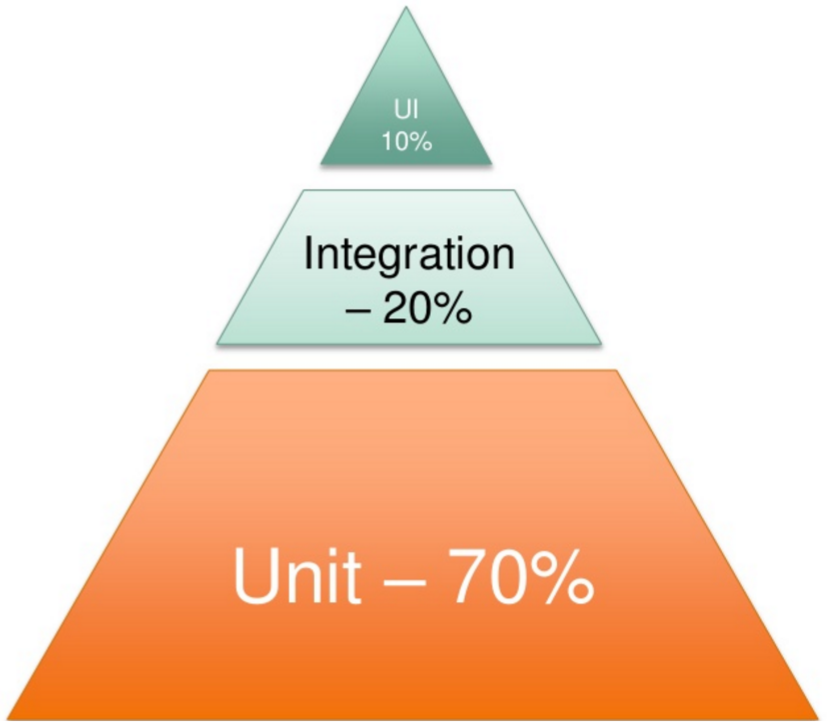
\includegraphics[width=0.6\textwidth]{testsProportions.png}
		\end{center}
	\end{frame}

\end{document}